\section{Working with Raster Data}\label{label_raster}
\index{raster layers|(}

QGIS supports a number of raster data formats. This section describes how to
work with raster data in QGIS.

\subsection{What is raster data?}\label{label_whatsraster}
\index{raster layers!definition}

Raster data in GIS are matrices of discrete cells that represent features on,
above or below the earth's surface. Each cell in the raster grid is the same
size, and cells are usually rectangular (in QGIS they will always be
rectangular). Typical raster datasets include remote sensing data such as
aerial photography or satellite imagery and modelled data such as an elevation
matrix.

Unlike vector data, raster data typically do not have an associated database
record for each cell.

In GIS, a raster layer would have georeferencing data associated with it which
will allow it to be positioned correctly in the map display to allow other
vector and raster data to be overlaid with it. QGIS makes use of georeferenced
rasters to properly display the data.\index{raster layers!georeferenced}
	
\subsection{Raster formats supported in QGIS}\label{label_rastformats}
QGIS supports a number of different raster formats. Currently tested formats
include:\index{raster layers!data formats}

\begin{itemize}
\item Arc/Info Binary Grid
\item Arc/Info ASCII Grid
\item GRASS Raster
\item GeoTIFF
\item Spatial Data Transfer Standard Grids (with some limitations)
\item USGS ASCII DEM
\item Erdas Imagine
\end{itemize}

Because the raster implementation in QGIS is based on the GDAL library, other
raster formats implemented in GDAL are also likely to work, but have not yet
been tested. See Appendix \ref{appdx_gdal} for more
details.\index{raster layers!GDAL implementation}
	
\subsection{Loading raster data in QGIS}\label{label_loadraster}


\includegraphics[width=0.7cm]{addraster} Raster layers
are loaded either by clicking on the \textsl{Load Raster} icon or by selecting the
\textsl{View~->~Add Raster Layer} menu option. More than one layer can be loaded at the
same time by holding down the Control key and clicking on multiple items in
the file dialog.\index{raster layers!loading}

Please refer to section \ref{sec:load_grassdata} if you intend to load GRASS rasterdata.
	
\subsection{Raster Properties Dialog}\label{label_rasterprop}

To view and set the properties for a raster layer, right click on the layer
name. This displays the raster layer context menu that includes a number of
items that allow you to:\index{raster layers!context menu}

\begin{figure}[ht]
   \begin{center}
   \caption{Raster context menu}\label{fig:raster_contextmenu}\smallskip
   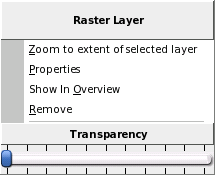
\includegraphics[clip=true, width=5cm]{rastercontextmenu}
\end{center}  
\end{figure}

\begin{itemize}
\item Zoom to the full extent of the raster
\item Zoom to the best scale of the raster
\item Show the raster in the map overview window
\item Remove the layer from the map
\item Open the raster layers properties
\item Rename the layer
\item Add a layer group
\item Expand legend tree view
\item Collapse legend tree view
\item Show file groups
\end{itemize}

Choose \textsl{Properties} from the context menu to open the raster properties
dialog for the layer.\index{raster layers!properties}

Figure \ref{fig:raster_properties} shows the properties dialog. There are five
tabs on the dialog: \textsl{Symbology}, \textsl{General}, \textsl{Metadata}, \textsl{Pyramids} and \textsl{Histogram}.

\begin{figure}[h]
   \begin{center}
   \caption{Raster Layers Properties
Dialog}\label{fig:raster_properties}\smallskip
   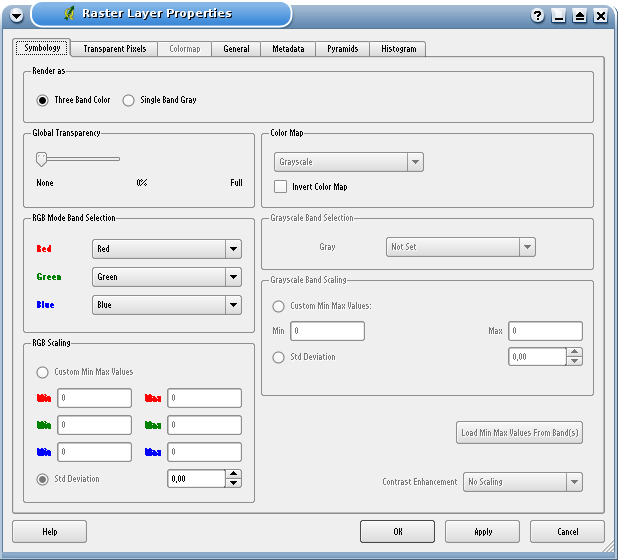
\includegraphics[clip=true, width=14cm]{raster_properties}
\end{center}  
\end{figure}

\subsubsection{Symbology Tab}\label{label_sombology}

QGIS supports three forms of raster layers:\index{raster layers!supported channels}

\begin{itemize}
\item Single Band Grayscale Rasters
\item Palette Based RGB Rasters
\item Multiband RGB Rasters
\end{itemize}

From these three basic layer types, eight forms of symbolised raster display
can be used:\index{raster layers!rendering interpretation}

\begin{itemize}
\item Single Band Grayscale
\item Single Band Pseudocolor
\item Paletted Grayscale (where only the red, green or blue component of the
image is displayed)
\item Paletted Pseudocolor (where only the red, green or blue component of the
image is displayed, but using a pseudocolor algorithm)
\item Paletted RGB
\item Multiband Grayscale (using only one of the bands to display the image)
\item Multiband Pseudocolor (using only one of the bands shown in
pseudocolor)
\item Multiband RGB (using any combination of three bands)
\end{itemize}

\smallskip

QGIS can invert the colors in a given layer so that light colors become dark
(and dark colors become light). Use the \textsl{Invert Color Map} checkbox to
enable / disable this behavior.\index{raster layers!icolor map inversion}

QGIS has the ability to display each raster layer at varying transparency
levels.\index{raster layers!transparency} Use the transparency slider to indicate to
what extent the underlying layers (if any) should be visible though the
current raster layer. 

QGIS can restrict the data displayed to only show cells whose values are
within a given number of standard deviations of the mean for the
layer.\index{raster layers!standard deviation} This is useful when you have one or
two cells with abnormally high values in a raster grid that are having a
negative impact on the rendering of the raster. This option is only available
for pseudocolor images.

\begin{Tip}\caption{\textsc{Viewing a Single Band of a Multiband Raster}}
\qgistip{If you want to view a single band (for example Red) of a multiband
image, you might think you would set the Green and Blue bands to ``Not
Set''. But this is not the correct way. To display the Red band, 
set the image type to grayscale, then select Red as the band to use for Gray.
}
\end{Tip} 

\subsubsection{General Tab}\label{label_generaltab}

The General tab displays basic information about the selected raster,
including the layer source and  display name in the legend (which can be
modified). This tab also shows a thumbnail of the layer, its legend symbol,
and the palette.\index{raster layers!properties}

Additionally scale-dependent visability can be set in this tab. You need to
check the checkbox and set an appropriate scale where your data will be
displayed in the map canvas.

Also the spatal reference system is printed here as a PROJ.4-string. 
This can be modified by hitting the \textsl{Change} button.

\subsubsection{Metadata Tab}\label{label_metatab}

The Metadata tab displays a wealth of information about the raster layer,
including statistics about each band in the current raster layer. Statistics
are gathered on a 'need to know' basis, so it may well be that a given layers
statistics have not yet been collected.\index{raster layers!metadata}


\begin{Tip}\caption{\textsc{Gathering Raster Statistics}}
\qgistip{To gather statistics for a layer, select pseudocolor rendering and
click the \textsl{Apply} button. Gathering statistics for a layer can be time
consuming. Please be patient while QGIS examines your
data!\index{raster layers!statistics}
}
\end{Tip}

\subsubsection{Pyramids Tab}\label{raster_pyramids}

Large resolution raster layers can slow navigation in QGIS. By creating lower
resolution copies of the data (pyramids), performance can be considerably
improved as QGIS selects the most suitable resolution to use depending on the
level of zoom.
\index{raster layers!pyramids}
\index{raster layers!resolution pyramids}

You must have write access in the directory where the original data is stored
to build pyramids. \\
Several resampling methods can be used to calculate the pyramides:
\begin{itemize}
\item Average
\item Nearest Neighbour
\item Average Magphase
\end{itemize}

Please note that building pyramids may alter the original data file and once
created they cannot be removed. If you wish to preserve a 'non-pyramided'
version of your raster, make a backup copy prior to building pyramids.

\subsubsection{Histogram Tab}\label{raster_histogram}

The histogram tab allows you to view the distribution\index{raster layers!histogram} 
of the bands or colors in your raster. You must first generate the raster statistics 
by clicking the \textsl{Refresh} button. You can choose which bands to display by 
selecting them in the list box at the bottom right of the dialog. Two different
chart types are allowed: Barcharts and Linegraphs.

Once you view the histogram, you'll notice that the band statistics have been
populated on the metadata tab.\index{raster layers!metadata)}

